
% --- PRIMO BLOCCO: Due immagini affiancate ---
\begin{figure}[htbp]
    \centering
    
    % Prima immagine (sinistra)
    \begin{subfigure}[b]{0.45\textwidth}
        \centering
        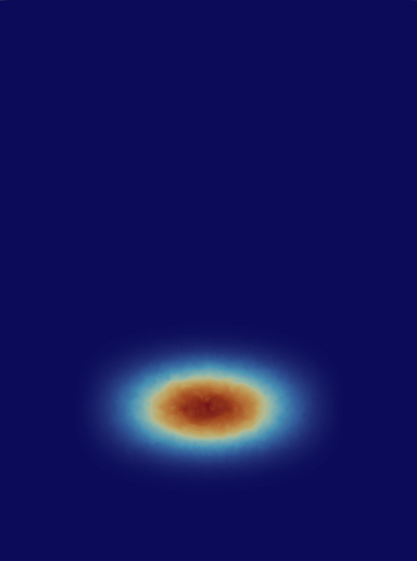
\includegraphics[width=\textwidth]{Giacomo/Foto_ground.png} 
        \caption{Ground state}
        \label{fig:foto1}
    \end{subfigure}
    \hfill 
    % Seconda immagine (destra)
    \begin{subfigure}[b]{0.45\textwidth}
        \centering
        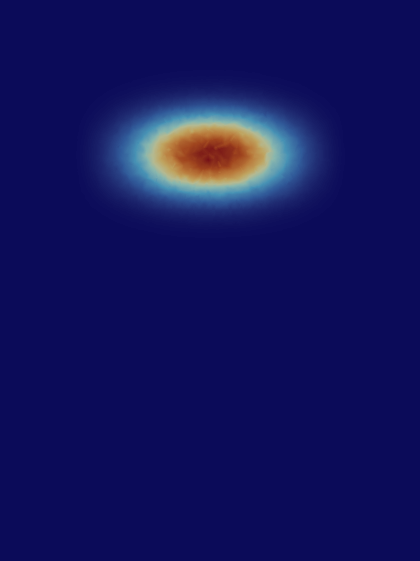
\includegraphics[width=\textwidth]{Giacomo/Foto_excited.png}
        \caption{First exited state}
        \label{fig:foto2}
    \end{subfigure}
    
    \caption{Soluzione dell'equazione di Shrodinger}
\end{figure}


% --- SECONDO BLOCCO: Immagine singola ---
\begin{figure}[htbp]
    \centering
    % Qui puoi decidere la larghezza della foto singola (es. 0.7 della pagina)
    \includegraphics[width=0.7\textwidth]{Giacomo/Densita_degli_stati.png}
    \caption{Soluzione dell'equazione di Shrodinger}
    \label{fig:foto3_sola}
\end{figure}
